\documentclass[presentation]{beamer}
\usepackage{common}
\usepackage{arydshln}

\newcommand{\cscat}[1]{$\langle\text{{\itshape#1}}\rangle$}
\newcommand{\csopt}[1]{{\itshape[#1]}}
\newcommand{\csalt}[1]{{\itshape(#1)}}
\newcommand{\op}[1]{\alert{`\texttt{#1}'}}
\newcommand{\operand}[1][\ldots]{{\normalcolor#1}}
\newcommand{\literal}[1]{\texttt{\alert{#1}}}
\newcommand{\bs}{$\backslash$}
\newcommand{\codepath}[1]{../../../code/lecture-02/#1}

\AtBeginSubsection[]
{
  \begin{frame}<beamer>
    \frametitle{Next In Line\ldots}
    \tableofcontents[currentsection,currentsubsection]
  \end{frame}
}

\title[\lecturecode{01}]{01 \\ \dotnet Fundamentals}

\author[Giovanni Ciatto]{Giovanni Ciatto\\\texttt{giovanni.ciatto@unibo.it}}

\begin{document}

\frame[label=coverpage]{\titlepage}

\section{\dotnet Overview}

\begin{frame}{What is \dotnet}
    \begin{block}{Definition}\centering
        \dotnet is a free, general-purpose, open-source, and multi-platform \emph{programming ecosystem}
    \end{block}  

    \vfill

    \begin{description}
        \item[programming ecosystem] | as it comprehends several languages, compilers, tools, libraries, etc.
        
        \vfill

        \item[multi-platform] | as it can be used on several OS and architectures (e.g. Win, Linux, MacOs, Android, etc)
        
        \vfill

        \item[open-source] | as its source code is publicly available and openly licensed
        
        \vfill

        \item[general-purpose] | as it supports several sorts of applications (e.g. desktop, mobile, web, videogames, databases, etc)
        
        \vfill

        \item[free] | as it is can be exploited with no additional costs
    \end{description}
\end{frame}

\begin{frame}[allowframebreaks]{\dotnet in a Nutshell}
    \begin{center}
        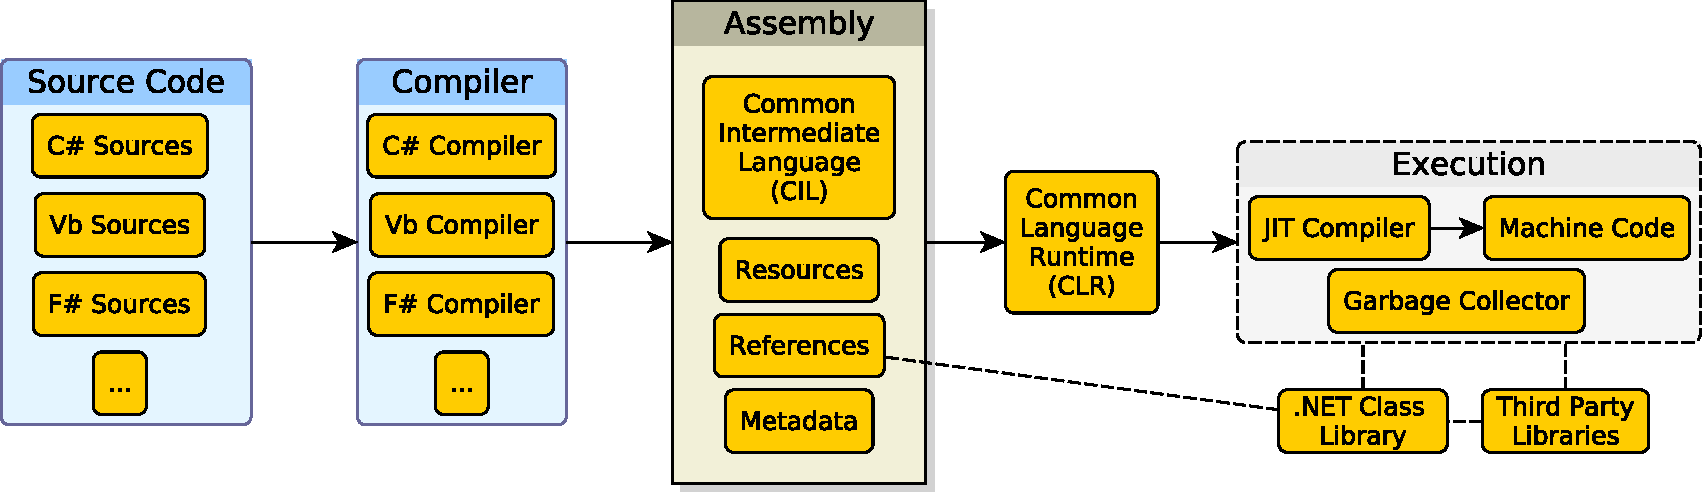
\includegraphics[width=\linewidth]{img/dotnet-overview.pdf}
    \end{center}

    \framebreak

    \begin{enumerate}
        \item Sources written using disparate \alert{languages} (e.g. \csharp, Vb, F\#, etc.)
        
        \smallskip

        \item can be compiled, via as many \alert{compilers}
        
        \smallskip

        \item into \alert{assemblies} containing
        %
        \begin{description}
            \item[common intermediate language (CIL)] |  a language- and platform-agnostic, compiled version of the sources
            \item[references] | dependencies declarations for the assembly
            \item[resources] | non-code files (e.g. internationalization strings, icons, default configurations, etc.) 
            \item[metadata] | for identifying the specific \emph{version} of the assembly
        \end{description}

        \smallskip
        
        \item which can then be executed by the \alert{common language runtime} (CLR) 
        %
        \begin{itemize}
            \item essentially, an \emph{interpreter} for the CIL
        \end{itemize}

        \smallskip

        \item  on any platform, via a \alert{just in time} (JIT) conversion into \alert{machine code}.
        
        \framebreak

        \item Execution of \dotnet code is \emph{managed} by default, meaning that:
        %
        \begin{itemize}
            \item developers must not take care of allocating/freeing memory
            \item as a \alert{garbage collector} is in charge of dynamically taking care of that
        \end{itemize}

        \bigskip

        \item \dotnet programs may reference (a.k.a. depend upon) other assemblies, such as
        %
        \begin{itemize}
            \item the \alert{\dotnet class library}, containing the standard SDK
            \item \alert{third party libraries}, either locally or remotely available
        \end{itemize}
        %
        and therefore exploit any class therein contained.

    \end{enumerate}
\end{frame}

\begin{frame}{\dotnet Platform -- The Present}
    \begin{center}
        \includegraphics[width=\linewidth]{img/dotnet-overview-present.png}
    \end{center}
\end{frame}

\begin{frame}{\dotnet Platform -- The Past}
    \begin{center}
        \includegraphics[width=\linewidth]{img/dotnet-overview-past.png}
    \end{center}
\end{frame}

\begin{frame}{\dotnet Platform -- Present vs. Past}
    \begin{itemize}
        \item Before \dotnet 5 there used to be three major implementations of the \emph{class library}:
        %
        \begin{description}
            \item[\dotnet Framework] | Windows-specific, full-featured, targetting desktop and web applications
            \item[\dotnet Core] | multi-platform (Win, Mac, Linux), less-featured, targetting desktop and web applications
            \item[Xamarin] | mobile-oriented (Android, iOS, Mac OS) 
        \end{description}

        \vfill

        \item Since \dotnet 5, implementations are aligned
    \end{itemize}

    \vfill

    \begin{alertblock}{In this course}\centering
        We stick to \alert{\dotnet Core 6.0}, to maximise interoperability and to avoid compatibility issues
    \end{alertblock}
\end{frame}

\section{Code Base Organization}

\subsection{Overview}

\begin{frame}[allowframebreaks]{Overview about Code Base Organization}
    \begin{center}
        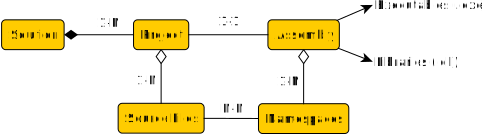
\includegraphics[width=\linewidth]{img/code-base.pdf}
    \end{center}

    \medskip

    \begin{enumerate}
        \item A \dotnet code base is called \alert{solution}
        
        \bigskip

        \item Each solution is a set of one or more related \alert{projects}
        %
        \begin{itemize}
            \item each project can contain sources written using a single \dotnet language
            \item different projects may target different \dotnet languages
            \item each project esplicitly targets one \emph{application model}
            %
            \begin{itemize}
                \item[eg] Class Library, Console/WinForms/WPF/Web Application, etc.
            \end{itemize}
        \end{itemize}

        \framebreak

        \item Each project is compiled into an \alert{assembly}
        %
        \begin{itemize}
            \item assemblies can either be executable or not---i.e. they can be \emph{libraries}
            \item executable assemblies have the \texttt{.exe} extension 
            \item library assemblies have the \texttt{.dll} extension
        \end{itemize}

        \medskip

        \item Each project is a container of several \alert{source} files 
        %
        \begin{itemize}
            \item containing several classes, structures, interfaces, or delegates definitions
            \item possibly organised into a number of \alert{namespaces}
        \end{itemize}

        \medskip

        \item Therefore, each assembly may \emph{expose} a number of namespaces, along with their definitions
    \end{enumerate}

    \bigskip

    \begin{block}{Takeway}\centering
        Assemblies (and therefore projects) are \emph{deployment} and \emph{execution} \alert{units}
    \end{block}
\end{frame}

\begin{frame}{Code Base Organization Enforcement}
    \begin{itemize}
        \item Tools (such as IDEs) \emph{enforce} such code base organization
        
        \bigskip

        \item You can expect all \dotnet-enabled tools to stick to this organization
        %
        \begin{itemize}
            \item[eg] Visual Studio (VS) or JetBrain Rider
        \end{itemize}

        \bigskip

        \item Analogies exists with other IDEs:
        \smallskip
        \begin{center}
            \begin{tabular}{c||c|c|c}
                & \textbf{VS/Rider} & \textbf{Eclipse} & \textbf{Idea} \\
                \hline\hline
                \textbf{Code Base}       & Solution          & Workspace        & Project       \\
                \hline
                \textbf{Deployment Unit} & Project           & Project          & Module       
            \end{tabular}
        \end{center}
    \end{itemize}
\end{frame}

\subsection{Directory Structure}

\begin{frame}[allowframebreaks]{Canonical Directory Structure of a \dotnet Solution}
    \begin{center}
        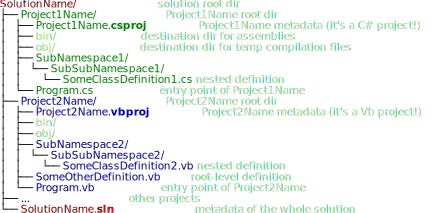
\includegraphics[width=\linewidth]{img/project-structure.pdf}
    \end{center}

    \framebreak

    \begin{itemize}
        \item Each solution $S$ has its own directory -- named $S$  -- containing:
        %
        \begin{itemize}
            \item a single \alert{$S$\texttt{.sln}} file
            \item a sub-directory for each project
        \end{itemize}

        \bigskip

        \item Each project $P$ has its own directory -- named $P$ --, within the solution directory, containing:
        %
        \begin{itemize}
            \item a single \alert{$P$\texttt{.csproj}} file (or $P$\texttt{.vbproj} for Vb projects)
            \item a directory for each namespace
            %
            \begin{itemize}
                \item possibly containing other sub-namespaces (and their directories)
                \item containing \texttt{.cs} source files (or \texttt{.vb} for Vb projects)
            \end{itemize}
            \item two directories, namely \texttt{bin/} and \texttt{obj/}, automatically generated
            \item some root-level \texttt{.cs} source files (or \texttt{.vb} for Vb projects)
        \end{itemize}

        \bigskip

        \item Conventionally, \emph{executable} projects contain a root-level \texttt{Program.cs} (or \texttt{.vb}) file
        %
        \begin{itemize}
            \item containing a \texttt{Main} method which is the \alert{entry proint} of the program
        \end{itemize}
    \end{itemize}
\end{frame}

\begin{frame}[allowframebreaks]{Example of \texttt{.sln} File}

    \lstinputlisting[basicstyle=\tiny\ttfamily]{\codepath{lecture-02.sln}}
    %
    \begin{itemize}
        \item[!] This is not somithing a developer may manually write!
    \end{itemize}
\end{frame}

\begin{frame}{Example of \texttt{.csproj} File}

    \lstinputlisting[basicstyle=\tiny\ttfamily]{\codepath{GreetingCLI/GreetingCLI.csproj}}
    %
    \begin{itemize}
        \item[!] This is not something a developer may comfortably manipulate!
    \end{itemize}
\end{frame}

\subsection{Handling a Solution}

\begin{frame}[allowframebreaks]{Handling a Solution via the Command Line}

    \begin{block}{The \texttt{dotnet} tool}
        \begin{itemize}
            \item All modern \dotnet installations comprehend a command-line tool named \alert{\texttt{dotnet}}
            \item It is the simpler way to handle a solution \emph{without} an IDE
            \item Among the many functionalities, it allows developers to:
            %
            \begin{enumerate}
                \item create a solution
                \item add projects to a solution
                \item compile a project into an assembly
                \item execute an executable assembly
                \item etc.
            \end{enumerate} 
        \end{itemize}
    \end{block}

    \begin{block}{How to use the \texttt{dotnet} tool}
        \begin{itemize}
            \item General syntax (square brackets denote optionality):
            %
            \begin{center}\centering\ttfamily\footnotesize
                \alert{\$} dotnet [sdk-options] [command] [command-options] [arguments]
            \end{center}

            \item How to learn how to use \texttt{dotnet}:
            %
            \begin{itemize}
                \item Run \texttt{dotnet [command] --help}
                \item See \url{https://docs.microsoft.com/dotnet/core/tools/dotnet}
            \end{itemize}
        \end{itemize}
    \end{block}

    \begin{exampleblock}{How to create \& manage a a solution with via \texttt{dotnet}}
        \begin{enumerate}
            \item Create a directory for the solution, say \texttt{MySolution}
            \item Open a shell into that directory
            \item Create an empty \texttt{.sln} file named after the current directory (i.e. \texttt{MySolution}):
            %
            \begin{itemize}\ttfamily
                \item[\$] dotnet new sln
            \end{itemize}
            \item Create a \csharp console app. project named \texttt{MyConsoleProject}:
            %
            \begin{itemize}\ttfamily\footnotesize
                \item[\$] dotnet new console -n MyConsoleProject -o MyConsoleProject
                \normalfont 
                \item[] (where \texttt{-n} indicates the project name, and \texttt{-o} its relative path) 
            \end{itemize}
            \item Register \texttt{MyConsoleProject} into \texttt{MySolution.sln}:
            %
            \begin{itemize}\ttfamily\footnotesize
                \item[\$] dotnet sln add MyConsoleProject/MyConsoleProject.csproj
                \normalfont 
                \item[] (recall to use \texttt{`\bs{}'} instead of \texttt{`/'} on Windows systems) 
            \end{itemize}    
            \item Run \texttt{MyConsoleProject} (re-compilation is implicit):
            %
            \begin{itemize}\ttfamily
                \item[\$] dotnet run --project MyConsoleProject/MyConsoleProject.csproj
            \end{itemize}
        \end{enumerate}
    \end{exampleblock}
    
\end{frame}

\begin{frame}[allowframebreaks]{Handling a Solution via the IDE}

    \begin{block}{Disclaimer}
        \begin{itemize}
            \item Using the command line may be hard, but it is free
            \item IDEs (e.g. Rider or VS) may be used instead, but they require a license
            \item We provide instructions for Rider, as it is multi-platform
            \item Apart for the appearance, VS is functionally very similar to Rider
            %
            \begin{itemize}
                \item as they rely on the same abstractions (solution, project, assembly, etc.)
            \end{itemize}
        \end{itemize}
    \end{block}

    \framebreak

    \begin{enumerate}
        \item Open your IDE
        %
        \begin{center}
            \includegraphics[width=.6\linewidth]{img/rider-1.png}
        \end{center}
        %
        (if you cannot see the welcome dialog above, then click on \alert{`File'} $\rightarrow$ \alert{`New\ldots'} to proceed)

        \framebreak

        \item Click on \alert{`New Solution'}
        %
        \begin{center}
            \includegraphics[width=.6\linewidth]{img/rider-2.png}
        \end{center}
        %
        \begin{enumerate}
            \item Choose the \emph{`Console Application'} template from the \emph{`\dotnet Core'} group
            \item Set the \emph{`Solution Name'} to \texttt{`MySolution'}
            \item Set the \emph{`Project Name'} to \texttt{`MyConsoleProject'}
            \item Ensure the \emph{`Solution Directory'} ends with \texttt{`MySolution'}
            \item Press the \alert{`Create'} button
        \end{enumerate}

        \framebreak

        \item The IDE should now appear like this:
        %
        \begin{center}
            \includegraphics[width=.6\linewidth]{img/rider-3.png}
        \end{center}
        %
        \begin{itemize}
            \item The \emph{Solution Explorer} view (here on the left) shows all the projects, along with their source files, dependencies (a.k.a. references), and resource files
            \item You can use that to browse the code base or you can \alert{Ctrl+Click} any symbol of any source file to jump to its definition
        \end{itemize}

        \framebreak

        \item You may use the \alert{`Play'} or \alert{`Bug'} button to run a project
        %
        \begin{center}
            \includegraphics[width=.6\linewidth]{img/rider-4a}
        \end{center}
        %
        \begin{itemize}
            \item The output of the program appears either below (Rider) or into a new window (VS)
            \item The `Play' appears close to the \texttt{Main} method as well
        \end{itemize}

        \framebreak

        \item Which project is actually run when you press `Play' depends on which project is currently selected:
        %
        \begin{center}
            \includegraphics[width=.6\linewidth]{img/rider-4b}
        \end{center}
        %
        \begin{itemize}
            \item Only \emph{executable} projects can be selected on that menu
            \item Recall that each executable project has a single \emph{entry point}
            %
            \begin{itemize}
                \item[ie] its \alert{\texttt{static void Main}} method
            \end{itemize}
        \end{itemize}

        \framebreak

        \item Assemblies may be compiled either in \alert{`Debug'} or in \alert{`Release'} mode:
        %
        \begin{center}
            \includegraphics[width=.6\linewidth]{img/rider-4c}
        \end{center}
        %
        \begin{itemize}
            \item When compiled in `Release' mode, optimisation are performed, which makes step-by-step debugging hard as some instructions may be pruned
            \item When compiled in `Debug' mode, no optiomisation is performed
        \end{itemize}

        \framebreak

        \item You may click close to a code line to set up a \alert{breakpoint} on that line
        %
        \begin{center}
            \includegraphics[width=.6\linewidth]{img/rider-5}
        \end{center}
        %
        \begin{itemize}
            \item breakpoints are \emph{ignored} when launching the program with `Play'
            \item breakpoints may \alert{suspend} a program execution, if it has been launched via the `Bug' button---i.e. in \alert{debug mode}
        \end{itemize}

        \framebreak
    
        \item While in debug mode, the program execution is suspended whenever the program \alert{reaches} a break point
        %
        \begin{center}
            \includegraphics[width=.6\linewidth]{img/rider-6}
        \end{center}
        %
        \begin{itemize}
            \item while suspended, you may \alert{inspect} the current status of a program execution
            %
            \begin{itemize}
                \item[eg] variables values, content of objects, call stacks, etc.
            \end{itemize}
            \item you may also make the program proceed \alert{step-by-step}
        \end{itemize}

    \end{enumerate}

\end{frame}

\begin{frame}[fragile]{Visual Studio Code}

\begin{itemize}
\item Microsoft's official \alert{.NET Extension pack}
\end{itemize}

\end{frame}

\section{Coding Conventions}

\begin{frame}[allowframebreaks]{About Coding Style Conventions}
    \begin{block}{Definition}
        \begin{itemize}
            \item Stylistic rules about how to write good-quality code
            %
            \begin{itemize}
                \item[eg] fields/properties/methods/types names, usage of white spaces, empty lines, comments, etc.
            \end{itemize}

            \item Usually \alert{followed} by all developers in a given community / project
            
            \item Possibily \alert{enforced} by \emph{automatic} tools
            
            \item Aimed at easing:
            %
            \begin{itemize}
                \item interoperability among developers,
                \item readability of the source code, and
                \item the maintainability of the code base
            \end{itemize}
        \end{itemize}
    \end{block}

    \begin{alertblock}{Coding Style Conventions are \textbf{Important}}
        \begin{itemize}
            \item Sticking to some \alert{shared} coding style is \emph{fundamental}
            %
            \begin{itemize}
                \item  especially, when working in \alert{teams}
            \end{itemize}
            
            \item Even if you are working alone, people may eventually join the project, forming a team
            %
            \begin{itemize}
                \item[$\rightarrow$] always act like you are in a team, even when coding alone
            \end{itemize}

            \item Coding conventions are \alert{not} a matter of \alert{taste}
            %
            \begin{itemize}
                \item \alert{do not ignore} some convention just because it appears \alert{ugly} to you
                \item conventions are never ugly/beautiful, nor right/wrong
                \item conventions are important as they are \alert{shared}
            \end{itemize} 

            \item One everybody gets used to conventions, they easy developers' understanding of the code
            %
            \begin{itemize}
                \item[eg] naming conventions help understanding what a symbol is without need to see its definition
                \item[$\rightarrow$] violating a convention is harmful: it misleads code readers  
            \end{itemize}
        \end{itemize}
    \end{alertblock}

    \begin{exampleblock}{\csharp Coding Conventions}\centering
        We stick to the conventions enumerated here:
        \\
        {\tiny \url{https://github.com/dotnet/runtime/blob/main/docs/coding-guidelines/coding-style.md}}
    \end{exampleblock}
    %
    \begin{itemize}
        \item[$\rightarrow$] we provide an overview of most relevant conventions in the next slides 
    \end{itemize}
\end{frame}

\begin{frame}[fragile,allowframebreaks]{\csharp Coding Style}

    \begin{block}{Concatenated Words Styles around the World}
        \begin{description}
            \item[\texttt{camelCase}] | \url{https://en.wikipedia.org/wiki/Camel_case}
            \item[\texttt{PascalCase}] | like \texttt{camelCase} but the first letter is uppercase
            \item[\texttt{snake\_case}] |  \url{https://en.wikipedia.org/wiki/Snake_case}
            \item[\texttt{kebab-case}] |  \url{https://it.wikipedia.org/wiki/Kebab_case} 
        \end{description}
        %
        \begin{itemize}
            \item[!] \dotnet conventions mostly rely on \texttt{camelCase} and \texttt{PascalCase}
        \end{itemize}
    \end{block}

    \begin{exampleblock}{Suggested Naming Conventions for \csharp}
        \begin{description}
            \item[\textbf{namespaces} names] are in \texttt{PascalCase} 

            \item[\textbf{type} names] (classes, interfaces, structures, delegates) are in \texttt{PascalCase}  
            %
            \begin{itemize}
                \item[eg] \texttt{String}, \texttt{List}, \texttt{Int32}, \texttt{Action} etc.
            \end{itemize} 

            \item[\textbf{inteface} names] start with a \texttt{`I'} and are in \texttt{PascalCase} 
            %
            \begin{itemize}
                \item[eg] \texttt{IList}, \texttt{ISet}, \texttt{IDictionary} etc.
            \end{itemize} 

            \item[\textbf{abstract class} names] start with \texttt{`Abstract'} and are in \texttt{PascalCase} 
            
            \item[\textbf{field} names] start with a \texttt{`\_'} and are in \texttt{camelCase} 
            
            \item[\textbf{method} names] are in \texttt{PascalCase} 
            
            \item[\textbf{property} names] are in \texttt{PascalCase} 
            
            \item[\textbf{local variables} and \textbf{methods parameters} names] are in \texttt{camelCase} 
            
        \end{description}
        %
        \begin{itemize}
            \item[!] all names are \alert{in English}
        \end{itemize}
    \end{exampleblock}

    \framebreak

    \begin{exampleblock}{Suggested Bracing Conventions for \csharp}
        \csharp bracing style is \alert{Allman's} one\footnote{\tiny(cf. \url{https://en.wikipedia.org/wiki/Indentation_style\#Allman_style})}
        %
        \begin{itemize}
            \item braces are always mandatory, except in single-line \alert{\texttt{if/else}} bodies 
            \item open and closed braces always lay their own line
            \item indentation levels of open/closed braces is the same of the clause they belong to
            \item statements within braces are subject to 4-spaces indentation
            \item[!] this style is different from Java's and JavaScript's ones
        \end{itemize}
\begin{lstlisting}
if (/* ... */)
{
    // something
}
\end{lstlisting}
    \end{exampleblock}

    \begin{exampleblock}{Suggested White Space Conventions for \csharp}
        \begin{itemize}
            \item Indentation exploits 4 spaces \alert{instead of} tabulations
            %
            \begin{itemize}
                \item you may need to enable white characters visualization to spot the difference
            \end{itemize} 
            \item A space is mandatory \alert{before and after} each \alert{infix} operator
            %
            \begin{itemize}
                \item[ie] arithmetic, boolean, bitwise, comparison operators, etc.
                \item[eg] \texttt{`a + b'} is ok, \texttt{`a!=b'} is not ok
            \end{itemize}
            \item Commas require \alert{no space before} and a \alert{single space after}
            %
            \begin{itemize}
                \item[eg] \texttt{`a, b'} is ok, \texttt{`a , b'} or \texttt{`a,b'} are not ok
            \end{itemize} 
            \item Semicolons require \alert{no space before} 
            \item Constructs require \alert{a single space} within name and round parenthesis opening
            %
            \begin{itemize}
                \item[eg] \texttt{`if (\ldots'}, \texttt{`while (\ldots'} or \texttt{`for (\ldots'} are ok
            \end{itemize} 
        \end{itemize}
    \end{exampleblock}

    \begin{exampleblock}{Other Suggested Conventions for \csharp}
        \begin{itemize}
            \item Define variables with \alert{\texttt{var}} only if the type is \alert{obvious and evident} in that context
            \item Use keywords instead of full names for built-in types (e.g., \lstinline|int| instead of \lstinline|System.Int32|)
            \item Define \alert{\texttt{readonly}} variables/fields/properties whenever possible (cf. \lstinline|final| in Java)
            \item Always specify visibility modifiers explicitly
            %\item Prefer conciseness when possible
            \item Order classes members as follows (top-down):
            %
            \begin{enumerate}
                \item fields
                \item constructors
                \item properties (public first)
                \item methods (public first)
                \item static members
            \end{enumerate}
        \end{itemize}
    \end{exampleblock}

    \begin{exampleblock}{Suggested File/Directory Organization for \dotnet}
        \begin{itemize}
            \item One type definition (class, struct, enum, delegate, \ldots) per file
            %
            \begin{itemize}
                \item so that developers may easily locate definitions
            \end{itemize}
            \item Name the file after the type definition it carries
            %
            \begin{itemize}
                \item[eg] \texttt{class Person} defined into \texttt{Person.cs} (or \texttt{Person.vb})
            \end{itemize}
            \item Each project exposes a \alert{root namespace} named after it
            %
            \begin{itemize}
                \item[eg] the root namespace of project \texttt{P} is named \texttt{P}
            \end{itemize}
            \item All source files from a project root directory contain type definitions laying within that project root namespace
            %
            \begin{itemize}
                \item[eg] the file \texttt{P/Person.cs} defines class \texttt{Person} within namespace \texttt{P}
            \end{itemize}
            \item Sub-directories reflect sub-namespaces
            %
            \begin{itemize}
                \item[eg] the file \texttt{P/People/Person.cs} defines class \texttt{Person} within namespace \texttt{P.People}
            \end{itemize}
        \end{itemize}
    \end{exampleblock}

\end{frame}

\begin{frame}{\csharp Coding Style -- Can you spot all the problems?}\centering

    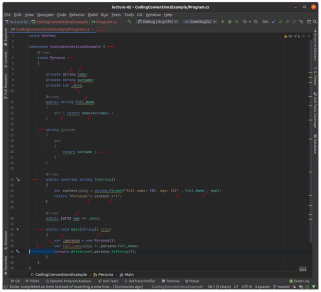
\includegraphics[width=0.7\linewidth]{img/wrong-conventions.png}

\end{frame}

\begin{frame}{\csharp Coding Style -- Can you name all the problems? }\centering

    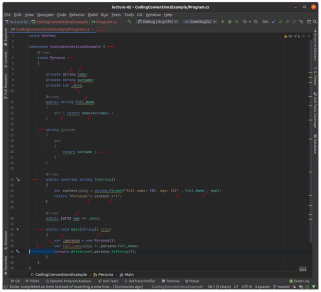
\includegraphics[width=0.7\linewidth]{img/wrong-conventions.pdf}

\end{frame}

\begin{frame}{\csharp Coding Style -- Correct Version }\centering

    \includegraphics[width=0.8\linewidth]{img/good-conventions.png}

\end{frame}

\end{document}
